\chapter{Annotation Guidelines}
\label{chap:annotation_guidelines}

Quality labelled annotated datasets are essential to build and evaluate argumentation
mining models.  High quality dataset annotation requires that annotators are
well trained in the task at hand. 
Data should be consistently annotated between indepedently working annotators. 
To ensure annotators understand the assigment and are able to complete 
the annotation task successfully, good annotation guidelines are required. 
During the annotation of data described in this thesis  
annotators had to do a test annotation before the real one, 
discuss differences until resolution, and redo annotation of examples
where there was no consensus. 
Once the annotation is complete, we measure inter-annotator agreement. 
In the case of two annotators that each classify $N$ items into $k$ mutually
exclusive categories, we use the Cohen's kappa \citep{cohen1960coefficient}. 
Cohen's kappa is defined as
$$
\kappa = \frac{p_0 - p_e}{1 - p_e}
$$
where $p_0$ is the relative observed agreement among annotators, and 
$p_e$ is the hypothetical probability of chance agreement. 
We use Fleiss' kappa to asses inter-annotator agreement when dealing with more than
two annotators \citep{fleiss1993review}.
Let $N$ be the number of annotators, $n$ number of ratings per subject, and
$k$ number of categories into which assignments are made. Then $n_{ij}$ represents
the number of annotators who assigned $i$-th subject to the $j$-th category. 
Fleiss' kappa is defined the same as Cohen's kappa, but $p_0$ and $p_e$ are defined as:
\begin{align*}
p_0 &= \frac{1}{Nn(n-1)} \left( \sum_{i=1}^{N} \sum_{j=1}^{k} n_{ij}^2 - Nn \right) \\
p_e &= \frac{1}{Nn} \sum_{j=1}^{k} \left( \sum_{i=1}^{N} n_{ij} \right)^2
\end{align*}

This chapter shows the annotation guidelines for 
\begin{enumerate*}[label=(\arabic*)]
\item microstructures (Section~\ref{sec:microstructure_annotation_appendix}), 
\item argumentative segments (Section~\ref{sec:argseg_annotation}),
\item prominent claim and claim relationship pairs (Section~\ref{sec:argrec_annotation}),
\item claim set similarities, (Section~\ref{app:sec:argpremises_annotation}), and
\item claim formalizations (Section~\ref{sec:formalization_annotation}).
\end{enumerate*}

\section{Microstructure annotation guidelines}
\label{sec:microstructure_annotation_appendix}

\noindent - Microstructures represent logically structured argumentative claims
\citep{boltuzic2017toward}. \\
- One can expresses logically equivalent claims in language \\
- To limit the language variation microstructures were designed to translate
expression rich phrases to be translated to a restricted language to allow for
easier inference \\
- microstructures  consist of domain specific concepts, 
connected through a finite set of argumentative relations, expressed using 
a certain modality \\
- microstructure annotation proceduced the microstructures data (
see item element in \ref{item:microstructures_dataset})\\

\newpage
\subsection{Cheat sheet}

\begin{minted}{microstructure_lexer.py:MicroStructureLexer -x}
viewpoint_1(
	viewpoint_2[holder](
		relation_1([quantity_1] concept_1, [quantity_2] concept_2)
	)
)

concept_1 = concept OR relation_2(concept_3, concept_4)
concept_2 = concept OR relation_3(concept_5, concept_6)

\end{minted}

\noindent \textbf{Viewpoints} \\
- Believes, Approves, Disapproves, Desires

\begin{minted}{microstructure_lexer.py:MicroStructureLexer -x}
viewpoint_1(
	relation_1(relation_2(concept_3, concept_4), concept_2)
)
\end{minted}

\noindent \textbf{Relations} (grayed columns indicate dual meaning between relations in each row)

\begin{table}[!htb]
\begin{tabular}{|c c c c c c|}
\hline
\cellcolor{gray!25} \texttt{promotes} & \cellcolor{gray!25}\texttt{allow} & \texttt{purpose} & \texttt{equal} & \cellcolor{gray!25}\texttt{entails}     & \texttt{has\_associated} \\
\cellcolor{gray!25} \texttt{suppress} & \cellcolor{gray!25}\texttt{deny}  &         &       & \cellcolor{gray!25}\texttt{contradicts} &  \\
\hline
\end{tabular}
\end{table}

\noindent \textbf{Negation} (use with relations)
Use with relation in front (\texttt{not\_promotes}, \texttt{not\_suppress}, \dots) \\
 
\noindent \textbf{Quantities} (use with concepts) \\
Some, All, Minority, Majority \\
          
\noindent \textbf{Concepts} 
\footnote{\url{https://docs.google.com/document/d/1ETobyCA4mpMmml1HXyxD7IG67EzrNK7W_2gzaIN0k_k/edit}} \\

\noindent \textbf{Quality} $\in [1, 5]$ \\
 
\noindent \textbf{Stance} $ \in {-2, -1, 0, 1, 2}$ \\

\pagebreak

\subsection{Task description}

In this task we annotate argumentative sentences/claims and represent them
using a logical generative grammar language, as well as a stance. The
argumentative sentences are paraphrases of debate post excerpts. We will
provide you with the original post, as the argumentative sentences provided
might not be enough to fully understand the meaning. 
The language has a set of syntactic rules, which need to be respected. The
syntax of your solutions will be checked as you annotate the document. 
An example sentence will look like:
\noindent\begin{tabular}{@{}lp{0.8\columnwidth}}
(ex. 1) & \textit{Homosexual marriage can not truly be a marriage.}
\end{tabular} \vspace{0.4cm}

\noindent We want to translate this to the form of: 

\begin{tabular}{@{}m{1.5cm}  m{4.5cm}}
(ex. 1) &  \begin{minted}{microstructure_lexer.py:MicroStructureLexer -x}
believes(
    contradicts(homosexual marriage, marriage)
)
\end{minted}
\end{tabular}

In this context, we call homosexual marriage and marriage concepts. The element
contradicts is a relation between the concepts. Believes is a viewpoint that
depicts the author's perspective. See more on concepts, relations and
viewpoints in the language description section below. 

Good practice when creating these annotations is attempting to read them back
in natural language. In this case, we get: I believe that homosexual marriage
is not marriage.  If we compare this to the original sentence, we see that it
captures the essence of the example sentence (ex. 1). The wording is lost,
which can mean a lot sometimes (reading between the lines), but this is
something we’re OK with.

\subsection{Language description}

As said, we annotate:
\begin{itemize}
\item Concepts
\item Relations between concepts
\item Viewpoints
\end{itemize}

\subsubsection{Concepts}

Concepts are noun phrases mentioned when discussing a topic. We provide a set
of concepts that we have previously identified for the ``gay rights'' topic\footnote{
Concepts available at 
\url{https://docs.google.com/document/d/1ETobyCA4mpMmml1HXyxD7IG67EzrNK7W_2gzaIN0k_k/edit?usp=sharing}
}
Some concepts are tab-shifted, which you can disregard, some have
slashes between them (i.e. \texttt{heterosexual marriage} / \texttt{traditional marriage}); we
consider these synonyms, please choose the first one. Your task is to search
through this list and find appropriate concepts (as close concept as possible)
mentioned in the input sentence and associate the appropriate relations between
them. Some example concepts: \texttt{procreation}, \texttt{reproduction}, \texttt{adoption}, \texttt{homosexual}
\texttt{adoption}, \texttt{have children}, \texttt{gay people}. 
If you feel you need to use a concept not
in the list, please contact us with the example. Another case would be where a
concept might be implicit, in the sentence: \textit{Allow gay marriages}, we recognize
the relation \texttt{allow} (explained in relations below) and the concept \texttt{gay marriages}
(argument B for relation \texttt{allow}).  We don’t know what the principle is, but from
the topic we know the state can allow gay marriages, therefore we can translate
the sentence as: \texttt{allow(state, gay marriage).}

\subsubsection{Quantity}

Each concept can be expressed with quantity. Quantities allowed are:
\begin{itemize}
\item Some 
\item All
\item Minority
\item Majority
\end{itemize}

\begin{table}[!htb]
\begin{tabular}{@{}m{1.5cm} m{5cm} m{8cm}}
\toprule
Example & Sentence & Microstructure \\
\midrule
(ex. 2.a) & Some people promote gay marriages. & 
\begin{minted}{microstructure_lexer.py:MicroStructureLexer -x}
believes(
  promote([some]people, gay marriage)
) 
\end{minted}
\\
(ex. 2.b) &Democracy helps the majority of people. &
\begin{minted}{microstructure_lexer.py:MicroStructureLexer -x}
believes( 
  promote(democracy, [majority] people)
)
\end{minted} 
\\
\bottomrule
\end{tabular}
\end{table}

\subsubsection{Relations}

Relations are connections between concepts. Relations are not domain-bound (one
can use them outside of gay marriages), while concepts are tied to domain 
(\texttt{gay marriages} in this case). Relations are verb phrases. 
Possible relations are:

\begin{footnotesize}
\begin{tabular}{lp{5cm}p{2.5cm}p{3cm}}
\toprule
Relation & Explanation & Argument A & Argument B \\
\midrule
\texttt{promotes(A, B)} & 
\makecell[cl]{
\textbf{A} promotes / fosters / \\
brings about / leads \\ 
/ forces / advances \\
/ increases /encourages \\
/ boosts / increases \\
the likelihood of / causes \textbf{B}  \\ \\
``Soft causation'' \\\\
\href{https://framenet2.icsi.berkeley.edu/fnReports/data/frameIndex.xml?frame=Cause_change_of_position_on_a_scale}{FrameNet link} 
}
& 
Agent (which promotes) & 
Attribute (what gets promoted) \\
\midrule
\texttt{suppress(A, B)} & 
\makecell[cl]{
\textbf{A} suppresses / decreases \\ 
likelihood / smothers / \\
represses / puts down / \\
vaniquishes \textbf{B} 
}
&
Agent (which suppresses) & 
Attribute (what gets suppressed)
\\
\midrule
\texttt{allow(A, B)} & 
\makecell[cl]{
Principle \textbf{A} \\ 
allows / approves / \\
licenses \textbf{B} \\\\
\href{https://framenet2.icsi.berkeley.edu/fnReports/data/frameIndex.xml?frame=Prohibiting_or_licensing}{FrameNet link}
} & 
Principle
& 
State of affairs \\
\midrule
\texttt{deny(A, B)} & 
\makecell[cl]{
Priciple \textbf{A} \\
denies / disallows /
bans \textbf{B} } & 
Principle & 
State of affairs\\
\midrule
\texttt{entails(A, B)} & 
\makecell[cl]{
State of affairs \textbf{A} \\
necessarily, per definition \\
or causally, makes \textbf{B} true \\\\
Proposition \textbf{B} has \\
support \textbf{A} \\\\
\href{https://framenet2.icsi.berkeley.edu/fnReports/data/frameIndex.xml?frame=Evidence}
{FrameNet link}
}
& State of affairs & Implication \\
\midrule
\texttt{contradicts(A, B)} & 
\makecell[cl]{
State of affairs \textbf{A} \\
makes \textbf{B} not true}
& State of affairs & Contradiction \\
\midrule
\texttt{purpose(A, B)} & 
\makecell[cl]{The purpose of \textbf{A} is \textbf{B} \\\\
\href{https://framenet2.icsi.berkeley.edu/fnReports/data/frameIndex.xml?frame=Purpose
}{FrameNet link}
} & Agent & Goal \\
\midrule
\texttt{has\_associated(A, B)} &
\makecell[cl]{
\textbf{A} has properties affected by \\
the existence of \textbf{B} \\\\
\href{https://framenet2.icsi.berkeley.edu/fnReports/data/frameIndex.xml?frame=Membership
}
{Similar FrameNet definition} 
} & Group & Member \\
\midrule
\texttt{equal(A, B)} & \textbf{A} is equal to \textbf{B} & Concept \textbf{A} & Concept \textbf{B} \\
\bottomrule
\end{tabular}
% \caption{Relation definition table}
% \label{tab:relation_definition}
% \end{table}
\end{footnotesize}

\subsubsection{Negation}
%TODO proper references in table rows

Relations can be negated to indicate opposite meaning. Notice how example $3.a$
is not saying it is suppressing, but just denied promoting. Example $3.b$ also can’t
use contradicts since being happy does not imply you are not rich, but it does
not imply you are.

\begin{footnotesize}
\begin{tabular}{@{}m{1.5cm} m{5cm} m{8cm}}
\toprule
Example & Sentence & Microstructure \\
\midrule
(ex. $3.a$) & \textit{Marijuana does not help cure cancer. } & 
\begin{minted}{microstructure_lexer.py:MicroStructureLexer -x}
believes(
  not_promotes(marijuana, cure cancer)
)
\end{minted}
\\
(ex. 3.b) & \textit{If you are happy, doesn’t mean you’re rich.} 
 &
\begin{minted}{microstructure_lexer.py:MicroStructureLexer -x}
believes(
  not_entails(feel happy, be rich)
)
\end{minted} 
\\
\bottomrule
\end{tabular}
\end{footnotesize}

\subsubsection{Nested Relations}

Relations can be nested within each other. Each relation takes two arguments.
An argument can be another relation or a concept. Make sure you are correct
with closing the opened braces. 

\begin{footnotesize}
\begin{tabular}{@{}m{1.5cm} m{5cm} m{8cm}}
\toprule
Example & Sentence & Microstructure \\
\midrule
(ex. $4.a$) & \textit{I think allowing gay marriages promotes freedom. } & 
\begin{minted}{microstructure_lexer.py:MicroStructureLexer -x}
believes(promotes(
  allow(state, gay marriage), freedom
  )
)
\end{minted}
\\
(ex. 4.b) & \textit{The purpose of life is to allow having freedom.} 
 &
\begin{minted}{microstructure_lexer.py:MicroStructureLexer -x}
believes(
  purpose(life, 
    allow(state, freedom)
  )
)
\end{minted} 
\\
(ex. 4.c) & \textit{It’s the same thing to allow gay marriages or heterosexual marriages.} & 
\begin{minted}{microstructure_lexer.py:MicroStructureLexer -x}
believes(
  equal(
    allow(state, gay marriage), 
    allow(state, heterosexual marriage)
  )
)
\end{minted}
\\
\bottomrule
\end{tabular}
\end{footnotesize}

\subsubsection{Viewpoints}

Viewpoints reflect whether the a viewpoint holder thinks the claim is believed
(fact), desired (policy), or considered right/wrong (value judgement). When not
mentioned, the claim holder is considered to be the author of the argumentative
sentence. If not, one needs to annotate the claim holder next to the viewpoint
type (\textit{I believe the Bible states}, \textit{I think the state of Florida should}), which
we call second-level viewpoints. Second-level viewpoints are annotated together
with a concept, for example: "\textit{I saw that the Bible states: It should be
allowed}" corresponds to "\texttt{believes(believes[Bible]...))}".
Possible viewpoints are \\

\begin{tabular}{l p{7cm} p{6cm}}
\toprule
Viewpoint & Description & Example \\
\midrule
\textbf{believes} & \textbf{A} believes / argues / thinks
that claim \textbf{C} is true & 
I believe people are mortal. \\
\midrule
\textbf{desires} & 
\textbf{A} believes / argues / thinks \textbf{C} 
should be true in the future or should remain true
& People should be nicer \\
\midrule
\textbf{approves} & 
\textbf{A} believes / argues / thinks \textbf{C} 
is morally / ethically right & Forgiving is bad \\
\midrule
\textbf{disapproves} & 
\textbf{A} believes / argues / thinks \textbf{C} 
is morally / ethically wrong & 
Drugs are bad.  \\
\bottomrule
\end{tabular} \\
% \label{tab:viewpoints}
% \caption{Viewpoints, their descriptions and examples of using specific viewpoints in claims}

\noindent Annotating a claim holder explicitly should be done like for sentence:

\begin{table}[h]
\begin{tabular}{@{}m{1.5cm} m{5cm} m{8cm}}
\toprule
Example & Sentence & Microstructure \\
\midrule
(ex. $5.a$) & \textit{I saw the Bible claims gay people are equal to straight people} & 
\begin{minted}{microstructure_lexer.py:MicroStructureLexer -x}
believes(
  believes[Bible](
    equal(gay people, straight people)
  )
)
\end{minted}
\\
\bottomrule
\end{tabular}
\label{tab:viewpoint_example}
\caption{Viewpoint claim annotation example}
\end{table}

\subsubsection{Stance}

Please annotate stance, which answers the question:
\textbf{Is the sentence pro-gay or not just by looking only at the offered claim} (not
the entire post context)? Stance $\in {-2, -1, 0, 1, 2}$.

\begin{table}[!htb]
\begin{tabular}{c p{10cm}}
\toprule
Stance Value & Explanation \\
\midrule
-2 & The author or the viewpoint of the second person is definitely against the
claim (explicitly states so). Any form of discrimination is seen as against.  \\
-1 & There is some implication that the author might be against gay rights  \\
0 & There is no stance towards gays, stance is bipolar \\
1 & Reverse of -1 \\
2 & Reverse of -2 \\
\bottomrule
\end{tabular}
\label{tab:stance}
\caption{Possible stance values with explanations}
\end{table}

\begin{table}[!htb]
\begin{tabular}{c p{10cm} r}
\toprule
Example & Claim & Stance \\
\midrule
(ex. $6.a$) &  I think allowing gay marriages promotes freedom. & 2 \\
(ex. $6.b$) & All people are equal. & 0 \\
(ex. $6.c$) & Allowing gay marriages will be the end of us all. &  -2 \\
(ex. $6.d$) & I would ban religious gay marriage. & -2 \\
(ex. $6.e$) & The Bible is against gay marriages & -2 \\
\bottomrule
\end{tabular}
\label{tab:stance_example}
\caption{Examples of stance for the gay marriages topic}
\end{table}

\subsubsection{Quality}

Evaluate your own logical claim transformation by inputting a number $\in [1, 5]$
rating how well does the proposed formalization suit what the person said?

\subsection{Technical instructions}

You will be provided with an excel spreadsheet with the posts and sentences.
Please notify us as soon as possible if you can’t use Excel - we can send you
the annotation in another format (Google spreadsheet, etc.). 

The goal is to fill up the E, F, G columns (logical representation, stance and
quality, highlighted in green) in the provided spreadsheet based on the
argumentative sentence in column D. Feel free to ignore columns A, and C (used
for internal tracking). Column B might be useful, if you can’t determine the
meaning in D. If you have problems or comments about an example, feel free to
add them in column H and raise questions with us -- we will be happy to
discuss! An example row will look like in table~\ref{tab:annotation_example}

\begin{table}[!htb]
\scriptsize
\begin{tabular}{|p{1.5cm} | p{2cm} | p{2cm} | p{2cm} | p{2cm} |c| c| c|}
\toprule
A & B & C & D & E & F & G & H \\
\midrule
POST ID & POST TEXT & SEGMENT ID & SENTENCE & LOGICAL REPRESENTATION
& STANCE & QUALITY & COMMENTS \\
\midrule
A75.data & 
Here we is the full text of the post. This will be relatively long.
This is divided into segments (argumentative sentences) that you then annotate. 
& 758 & 
The full text of the post will be relatively long.  
& \cellcolor{green!25} &  \cellcolor{green!25}& \cellcolor{green!25} & \cellcolor{green!25} \\
\bottomrule
\end{tabular}
\caption{Example excel sheet to annotate}
\label{tab:annotation_example}
\end{table}

A syntax checking script and your annotation is packaged into a zip file.  Your goal is to
fill column E in \texttt{annotation.xls}.

\subsubsection{Checking syntax correctness (optional)}

We provide a script to verify that your solutions are syntactically correct. 
You will need to install python and a python library xlrd. Make sure to install
\texttt{python 2.x}!

If you are not familiar with python, installing them on Windows is desribed in
\url{http://www.howtogeek.com/197947/how-to-install-python-on-windows/}
Xlrd is available to install from:
\url{http://www.lexicon.net/sjmachin/xlrd-0.6.1.win32.exe} 
To install it, you will need to Run-as-administrator. 
Please contact us if you have issues installing these. 
To help check correctness of your solution, we offer a python script that can
be run in two ways:

\begin{description}[style=multiline, labelwidth=1.5cm]
\item[\namedlabel{item:excel}{All}] Check all solutions in your excel spreadsheet
\item[\namedlabel{item:single_claim}{Single}] Check a single claim
\end{description}

\begin{figure}
	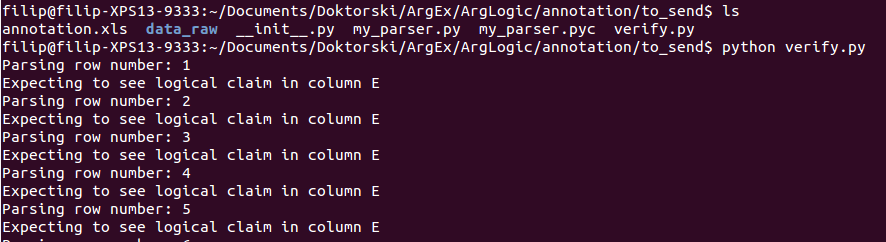
\includegraphics[scale=0.5]{struc_instructions_1.png}
	\caption{Expected output of running microstructure syntax check on entire file (\ref{item:excel}) mode}
	\label{fig:struc_instructions_all}
\end{figure}

\begin{figure}
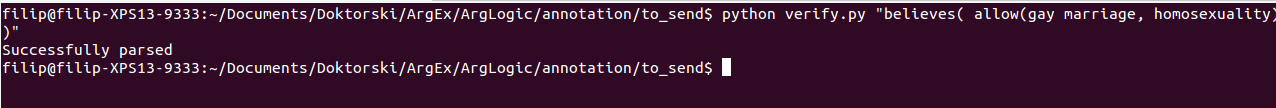
\includegraphics[scale=0.35]{struc_instructions_2.png}
	\caption{Expected output of running microstructure syntax check on a
	\label{fig:struc_instructions_2}
	single claim (\ref{item:single_claim} mode) }
\end{figure}

\noindent The script and your annotation is packaged into a zip available here. When you
unzip it, you should input your solutions in excel file \texttt{to\_send/annotation.xls}
To run it in \ref{item:excel} mode simply run \texttt{python verify.py} while
positioned in the \texttt{to\_send} directory using the command line (shown in
figure~\ref{fig:struc_instructions_all}) To run in \ref{item:single_claim}
mode, also position yourself in the \texttt{to\_send/} directory, but run as
shown in figure~\ref{fig:struc_instructions_2}.


\section{Claim segment annotation}
\label{sec:argseg_annotation}

Annotating claim segments from user comments splits the comment into claims. The
claims can be transformed into microstructures (as done to create the
microstructure dataset described in~\ref{item:microstructures_dataset}) or
formalized structures (as done to create the argument structure dataset
described in~\ref{item:structure_dataset}). Annotating segments involves
paraphrasing extracted segments to help streamline the annotation of segments
to structures. 

The task is to segment debate posts into claims. Each annotator gets a sheet in
a Google Sheets file with their name.  Column $C$ contains a user comment on
the topic of ``\textit{Should marijuana be legal}'' (MA).  The annotator needs
to carefully read the user comment, determine the stance of the comment along
with the explicit and implicit claims upon which the comment founds the
expressed stance. 

For each comment, the annotation involves:
\begin{enumerate}
\item extracting all argumentative segments of the comment as an atomic claim,
\item labeling the type of extracted segments, and
\item creating a paraphrase of the extracted segment.
\end{enumerate}
All argumentative segments should be copied to column $D$. 
Each extracted segment needs to be marked with an integer which denotes the
ordering of appearance in the post (segment $S1$, $S2$, $S3$, \dots)
All text belonging to segment $S1$ needs to be copied to column $D$, whereas
the original comment text needs to be edited to mark the segments belonging to 
the extracted segments. The beginning and end 
of the segment $Sx$ need to be marked with \texttt{<Sx>} and \texttt{</Sx>} respectively. 
Discontiguous segments are also allowed, they need to be marked with start and end tags
for each segment. Copying discontiguous segments is done by concatenating all 
instances in order of appearance. 
Column $E$ needs to contain the segment 
identifier ($S1$, $S2$, \dots). Please note that each start tag needs to be
paired with an end tag. 

\noindent Example 1: 

\begin{itemize}
  \item[] Comment: ``People are great, they have many virtues.''
  \item[] Segment $S1$: ``People are great''
  \item[] Segment $S2$: ``they have many virtues''
  \item[] Edited comment: ``\texttt{<S1>}People are great\texttt{</S1>},
  \texttt{<S2>}they have many virtues\texttt{</S2>}. ''
\end{itemize}

\noindent Example 2:
\begin{itemize}
\item[] Comment: ``People are smart and stupid.''
\item[] Segment $S1$: ``People are smart''
\item[] Segment $S2$: ``People are stupid''
\item[] Edited comment: ``\texttt{<S1><S2>}People are\texttt{</S2>} smart\texttt{</S1>}
and \texttt{<S2>}stupid\texttt{</S2>}''
\end{itemize}

\subsection*{Argumentative segment type}

The extracted segment needs to have a labelled segment type in column $F$ of
the Google sheets document. The segment needs to be classified according to two
taxonomies. First, the segment needs to be classified as either a 
\begin{enumerate}
\item fact --- statement that is true or untrue,
\item policy --- statement providing a solution or another series of questions in response to a fact,
\item value --- judgement, appraisal or evaluation. 
\end{enumerate}
Second, the segment needs to be labelled as either a 
\begin{enumerate}
\item assertion --- explicit statement or announcement or
\item rhetorical question --- question not expecting an answer. 
\end{enumerate}
More on facts, values and policies \citep{factvaluepolicy}.

\subsection*{Segment paraphrase annotation}

For each extracted segment, a paraphrase needs to be constructed. The paraphrase needs to
be assigned to column $G$ in spirit of the following principles:
\begin{itemize}
\item \textbf{Argumentativeness} -- Only argumentative text should be paraphrased; 
\item \textbf{Atomicity} -- A claim should convey a single thought; 
\item \textbf{Authority} -- Experts in claims from expert opinion should be made explicit in the paraphrase; 
\item \textbf{Brevity} -- Paraphrases should keep only the relevant argumentative content; 
\item \textbf{Canonicity} -- Canonical terms and phrases are preferred over idiomatic language;
\item \textbf{Contextuality} -- Claims should be paraphrased by considering their local and
topical context as well as their context;
\item \textbf{Declarativity} -- paraphrases should 
be in declarative form;
\item \textbf{Dereferencing} -- Pronouns and nominal  references
should be  resolved;  and
\item \textbf{Explicitness} -- Only explicitly stated
information should be paraphrased, and not whatever might be implied by the claim
\end{itemize}

\subsection*{Examples of segment annotation}

\begin{mydef}
By banning gay adoption, children in gay couple households have no legal status
should something happen to the parents, including death or serious illness.
The child cannot claim inheritances or other household assets in case of death.
If one parent dies, the second parent has no legal right to take custody or
care for the child.   A parent without legal right to a child cannot legally
register him/her for school.   Parents cannot put children on some health
insurance plans.   Parents cannot make medical decisions for the child.   * The
child has no claim to the social security or other insurance benefits of the
parent.   Gay couple parents without adoption rights do not benefit from the
generous tax deductions granted to heterosexual parents.
\end{mydef}

\noindent Extracted segments:
\begin{itemize}
\item[] \textbf{Segment1:} ``By banning gay adoption, children in gay couple
households have no legal status should something happen to the parents,
including death or serious illness.''
\item[] \textbf{Type}: Fact, assertion
\item[] \textbf{Paraphrase}: ``Children without a legal status are not
protected in case something happens to their parents''
\end{itemize}

\begin{itemize}[topsep=0.3cm]
\item[] \textbf{Segment2}: ``The child cannot claim inheritances or other household assets in case of death.''
\item[] \textbf{Type}: Fact, assertion
\item[] \textbf{Paraphrase}: ``Children without a legal status cannot claim
inheritance or other household assets in case of death.''
\end{itemize} 

\begin{itemize}[topsep=0.3cm]
\item[] \textbf{Segment3}: ``If one parent dies, the second parent has no legal
right to take custody or care for the child.''
\item[] \textbf{Type}: fact, assertion
\item[] \textbf{Paraphrase}: ``If one parent dies, the second parent has no legal
right to take custody or care for the child.'' (same)

\end{itemize}

\begin{itemize}[topsep=0.3cm]
\item[] \textbf{Segment4}: ``A parent without legal right to a child cannot
legally register him/her for school.''
\item[] \textbf{Type}: fact, assertion
\item[] \textbf{Paraphrase}: ``A parent without legal right to a child cannot
legally register him/her for school.'' (same)
\end{itemize}

\begin{itemize}[topsep=0.3cm]
\item[] \textbf{Segment5}: ``Parents cannot put children on some health insurance plans.''
\item[] \textbf{Type}: fact, assertion
\item[] \textbf{Paraphrase}: ``Parents cannot put children on some health insurance plans.'' (same)

\end{itemize}

\begin{itemize}[topsep=0.3cm]
\item[] \textbf{Segment6}: ``Parents cannot make medical decisions for the child.''
\item[] \textbf{Type}: fact, assertion
\item[] \textbf{Paraphrase}: ``Parents cannot make medical decisions for the child.''
\end{itemize}

\begin{itemize}[topsep=0.3cm]
\item[] \textbf{Segment7}: ``The child has no claim to the social security or
other insurance benefits of the parent''
\item[] \textbf{Type}: fact, assertion
\item[] \textbf{Paraphrase}: ``The child has no claim to the social security or
other insurance benefits of the parent''
\end{itemize}

\begin{itemize}[topsep=0.3cm]
\item[] \textbf{Segment8}: ``Gay couple parents without adoption rights do not
benefit from the generous tax deductions granted to heterosexual parents.''
\item[] \textbf{Type}: fact, assertion
\item[] \textbf{Paraphrase}: ``Unmarried gay parents cannot claim adoption rights
to benefit from tax deductions.''
\end{itemize}

\begin{mydef}
No it shouldnt be allowed. Marriage is when man and women get married. In the
Bible it says that its a sin for marrying your same gender and its a immoral
sin. Look at the animals they have one male and one female you dont see 2 male
horse with each other or any other animals. Look at the example animals make
learn from them.
\end{mydef}

\begin{itemize}[topsep=0.3cm]
\item[] \textbf{Segment1}: it shouldnt be allowed
\item[] \textbf{Type}: policy, assertion
\item[] \textbf{Paraphrase}: Gay marriage should not be allowed.
\end{itemize}

\begin{itemize}[topsep=0.3cm]
\item[] \textbf{Segment2}: Marriage is when man and women get married.
\item[] \textbf{Type}: fact, assertion
\item[] \textbf{Paraphrase}: Marriage is between a man and a woman.
\end{itemize}

\begin{itemize}[topsep=0.3cm]
\item[] \textbf{Segment3}: In the Bible it says that its a sin for marrying your same gender and its a immoral sin.
\item[] \textbf{Type}: fact, assertion
\item[] \textbf{Paraphrase}: According to the bible, same-sex marriage is immoral.
\end{itemize}

\begin{itemize}[topsep=0.3cm]
\item[] \textbf{Segment4}: Look at the animals they have one male and one female
\item[] \textbf{Type}: fact, assertion
\item[] \textbf{Paraphrase}: Animals of opposite sex pair up.
\end{itemize}

\begin{itemize}[topsep=0.3cm]
\item[] \textbf{Segment5}: you dont see 2 male horse with each other or any other animals
\item[] \textbf{Type}: fact, assertion
\item[] \textbf{Paraphrase}: Animals of same sex do not pair up.
\end{itemize}

\begin{itemize}[topsep=0.3cm]
\item[] \textbf{Segment6}: Look at the example animals make learn from them.
\item[] \textbf{Type}: policy, assertion
\item[] \textbf{Paraphrase}: We should learn from how animals behave.
\end{itemize}

\subsubsection*{Segment atomicity}

\begin{mydef}
I do not at all feel as God wants two men or two woman to be together, as he
has made each a man and a woman to combine and be together. However, it is our
constitutional right to make our own chices in America. What I believe should
be "exit only" is non of my business where people put things. As far as a legal
bond, we are considered "one nation under God" but , the goverment would make a
benifit from gay marriage, wether I a gree or not. Like I said we should have
the freedom to choose, we are Americans and our ancestors fought for our
freedom!!!!! Hey and I hope everyone is fighting to keep seatbelts a
choice,please keep fighting for our FREEDOM of choice!!!
\end{mydef}
This extracted segment expresses two separate ``thoughts''
\begin{itemize}
\item[] ``What I believe should be "exit only" is non of my business where people put
things.''
\end{itemize}
therefore it should be divided into two segments:
\begin{itemize}
\item[]  ``I believe should be "exit only"''
\item[] ``is non of my business where people put things''
\end{itemize}

\subsection*{Assuming too many implicit premises}

\begin{mydef}
I do not at all feel as God wants two men or two woman to be together, as he
has made each a man and a woman to combine and be together. However, it is our
constitutional right to make our own chices in America. What I believe should
be "exit only" is non of my business where people put things. As far as a legal
bond, we are considered "one nation under God" but , the goverment would make a
benifit from gay marriage, wether I a gree or not. Like I said we should have
the freedom to choose, we are Americans and our ancestors fought for our
freedom!!!!! Hey and I hope everyone is fighting to keep seatbelts a
choice,please keep fighting for our FREEDOM of choice!!!
\end{mydef}
The segment ``our ancestors fought for our freedom'' can be understood
such that the author believes that freedom refers to the freedom of choice.
This might be the case, but concluding so requires making assumptions based 
derived on implicit premises. 

\begin{itemize}
\item[] ``American ancestors fought for freedom to choose''
\end{itemize}
This paraphrase assumes ``freedom to choose''. But, the same segment can be
paraphrased not to include implicit knowledge and paraphrase in the following way 
(while also dereferencing the pronoun ``our'' to ``Americans''):
\begin{itemize}
\item[] ``Ancestors of current Americans fought for freedom of Americans.''
\end{itemize}

\subsection*{Reusing segment parts}

\begin{mydef}
As you say, "Marriage is something in particular." Its a legal union requiring
a license from a government office, not from a religious organization. That's
why gay people are fighting for "equal rights", not "equal rites."   For the
government to remain neutral on this issue, they need to stop denying gay
people the same rights as others to marry. As it is, the federal government is
anything but neutral. They deny over one thousand federal benefits to people
legally married in several states who happen to be of the same sex.
\end{mydef}
One candidate segment to extract would be:
\begin{itemize}
\item[] ``For the government to remain neutral on this issue, they need to stop
denying gay people the same rights as others to marry''
\end{itemize}
This segment actually contains three connected atomic segments (in paraphrased form):
\begin{itemize}
\item[] ``The government needs to remain neutral on this issue''
\item[] ``The government needs to stop denying gay people rights to marry''
\item[] ``Everyone but gay people have the rights to marry''
\end{itemize}


\begin{mydef}
This is the dictionary definition of marriage:   a.   the social institution
under which a man and woman establish their decision to live as husband and
wife by legal commitments, religious ceremonies, etc. Antonyms: separation.
b.   a similar institution involving partners of the same gender: gay marriage.
Antonyms: separation.   2.   the state, condition, or relationship of being
married; wedlock: a happy marriage. Synonyms: matrimony. Antonyms: single life,
bachelorhood, spinsterhood, singleness; separation.   3.   the legal or
religious ceremony that formalizes the decision of two people to live as a
married couple, including the accompanying social festivities: to officiate at
a marriage. Synonyms: nuptials, marriage ceremony, wedding. Antonyms: divorce,
annulment.   4.   a relationship in which two people have pledged themselves to
each other in the manner of a husband and wife, without legal sanction: trial
marriage.   5.   any close or intimate association or union: the marriage of
words and music in a hit song. Synonyms: blend, merger, unity, oneness;
alliance, confederation. Antonyms: separation, division, disunion, schism.
There is no mention of the reason for marriage being to Pro-create, the only
reason people should get married should be because they love each other and if
two Gay people love each other they should be allowed to marry. You can
Pro-create without getting married and I know many straight married people who
dont have Children they married because they loved each other not to have
children and Gay people should be allowed this right as well
\end{mydef}
Segment ``many straight married people who dont have Children they married
because they loved each other not to have children''
can be divided into three atomic segments:
\begin{itemize}
\item[] ``many straight married people who don't have Children''
\item[] ``many people married because they loved each other''
\item[] ``many people married not to have children''
\end{itemize}

\subsection*{Recognizing value segments}

Value segments often involve explicitly judging the value of an object.
Sometimes, the judgement can be made implicitly, but seeing explicit 
expressions should be preffered. For example: 
``People argue Gay marriage will lead to and allow
nontraditional families.'' is a factual statement, because 
the author expresses his views of public opinion. If the author expressed
his personal view like ``gay marriages lead to nontraditional families''
this could be considered a value statement, with the key part being
the word ``nontraditional'' which expresses negativity towards ``gay marriages''.
Whether there is a another view holder can influence the segment type. 
The segment ``The bible says Gay rights are immoral'' is considered a factual statement, 
whereas the segment ``Gay rights are immoral'' is considered to be a 
value segment since the segment is attributed to the author. 


\section{Prominent Claim Identification Annotation}
\label{sec:argrec_annotation}

Prominent claim identification is the task of recognizing which (from a set of
predefined) prominent claims is mentioned in a target comment and how. The goal
of the task is to label prominent claim-comment pairs with a label:
\begin{itemize}
	\item \textbf{A} -- explicitly attacks the prominent claim
	\item \textbf{a} -- vaguely/implicitly attacks the prominent claim
	\item \textbf{N} -- makes no use of the prominent claim
	\item \textbf{s} -- vaguely/implicitly supports the prominent claim
	\item \textbf{S} -- explicitly supports the prominent claim
\end{itemize}
Labeling the dataset according the guidelines below
produced the \ComArg dataset (described in section~\ref{sec:comarg}.

\subsection*{Annotation Guidelines}

There is an online discussion about ``gay rights''. The topic is ``SHOULD GAY
PEOPLE BE ALLOWED TO MARRY?''. Users post comments on the discussion forum,
which express opinions that are either for or against gay marriages. For
example: COMMENT: ``Gay people shouldn’t marry because they can’t have
children.''
In these discussions, users often refer to certain well-established arguments .
For example, typical arguments are:
\begin{itemize}
\item ARGUMENT 1: ``All people should be treated equally.''
\item ARGUMENT 2: ``Marriage should be between two believers who can produce godly offspring.''
\item ARGUMENT 3: ``Marriage is about more than procreation, therefore gay couples should not be denied the right to marry due to their biology.''
\end{itemize}

\noindent Your task is to detect WHICH arguments are used in a comment and HOW. You will
be presented with three arguments for each comment. For each argument, there
will be five check boxes, numbered 1 (DENIED) through 5 (APPROVED). 

\noindent For each argument, you need to do the following:
\begin{itemize}
\item if the comment directly denies the argument, check 1 (DENIED).
\item if the comment does not refer to the argument, check 3 (NOT MENTIONED)
\item if the comment approves the argument to make its point, check 5 (APPROVED).
\end{itemize}

\noindent You might feel that the comment approves or denies the argument, but you're not
completely certain. If you think that the argument is indirectly or partially
denied, check option 2, which is the option between DENIED and NOT MENTIONED.
Conversely, if you think that the argument is indirectly or partially approved,
check option 4, which is the option between NOT MENTIONED and APPROVED.
Note that it will often be the case that an argument is not mentioned.

Also note that if a comment and an argument express a different opinion, it
does not automatically mean that the argument is denied. For example, a comment
``Marriage is a religious institution, and the major world religions frown upon
homosexuality'' does not deny the argument ``Gay couples should be able to take
advantage of the fiscal and legal benefits of marriage''. Here, the comment and
the argument do express different opinions over the issue, but the argument
itself is not mentioned in the comment.

Consider again the example above. To detect whether and how ARGUMENTS 1-3 are
used in COMMENT, think in the following way.
In case of ARGUMENT 1: ``All people should be treated equally.''

\begin{enumerate}
\item    ARGUMENT 1 refers to human equality
\item    COMMENT does NOT refer to human equality
\item    Therefore, check option 3 (NOT MENTIONED) for ARGUMENT 1.
\end{enumerate}

\noindent In case of ARGUMENT 2: ``Marriage should be between two believers who can
produce godly offspring.''

\begin{enumerate}
\item ARGUMENT 2 implies that having children is a necessary condition for
marriage
\item COMMENT states that gay people shouldn’t marry because they cannot have
children, implying that having children is a necessary condition for marriage
\item BOTH claims are about having children and make the same point
\item therefore, COMMENT supports ARGUMENT 2
\item check option 5 (APPROVED)
\end{enumerate}

\noindent In case of ARGUMENT 3: ``Marriage is about more than procreation, therefore gay
couples should not be denied the right to marry due to their biology.''

\begin{enumerate}
\item ARGUMENT 3 implies that having children is not a necessary condition for marriage
\item COMMENT states that gay people shouldn’t marry because they cannot have children, implying that having children is a necessary condition for marriage
\item BOTH claims are about ``having children'', but COMMENT states the opposite of ARGUMENT 3
\item therefore, COMMENT denies ARGUMENT 3
\item check option 1 (DENIED)
\end{enumerate}


\section{Implicit claim annotation}
\label{app:sec:argpremises_annotation}

\subsection*{Annotation guidelines}

%This produced the argpremises dataset similarities in the (\ref{item:argpremises}).

IMPORTANT: This is essentially a reading comprehension task. While we
appreciate your opinion on this topic, this task is about analyzing OTHER
PEOPLE'S OPINIONS, not expressing your own. This is not an online survey.

\noindent There is an online discussion on marijuana legalization. The topic is: ``SHOULD
MARIJUANA BE LEGALIZED?''. You have to be familiar with of the issue: You can
get basic information about the topic 
in the footnotes\footnote{\url{http://medicalmarijuana.procon.org/}}\footnote{
\burl{http://idebate.org/debatabase/debates/health/addiction/
house-believes-cannabis-should-be-legalised}
}
Your goal is to identify whether the two sentences offered are talking about
the same thing. Please rate the SIMILARITY LEVEL for each pair of sentences:
\begin{itemize}
\item 6: very similar
\item 5 or 4: somewhat similar
\item 3 or 2: somewhat dissimilar
\item 1: not similar
\end{itemize}

\noindent Example one:
\begin{table}[h!]
\begin{tabular}{|@{\ }r@{\ \  }p{0.72\columnwidth}|}
\hline
\textbf{Sentence 1:} & \emph{Marijuana does not cause any damage to our bodies}\\
\textbf{Sentence 2:} & \emph{Consuming pot never hurt anyone}\\
\textbf{Similarity level} & 6 \\
\hline
\end{tabular}
\end{table}
\pagebreak
%\caption{User claim, the matching main claim, and the implicit premises filling the gap.}

\noindent Example two:
\begin{table}[h!]
\begin{tabular}{|@{\ }r@{\ \  }p{0.72\columnwidth}|}
\hline
\textbf{Sentence 1:} & \emph{If legalized, people will use marijuana and other drugs more}\\
\textbf{Sentence 2:} & \emph{Marijuana can be used as medicine because it showed positive effects}\\
\textbf{Similarity level} & 1 \\
\hline
\end{tabular}
\end{table}

\noindent Example three:
\begin{table}[h!]
\begin{tabular}{|@{\ }r@{\ \  }p{0.72\columnwidth}|}
\hline
\textbf{Sentence 1:} & \emph{A large portion of modern music an art has been inspired by marijuana}\\
\textbf{Sentence 2:} & \emph{Used as a medicine for its positive effects}\\
\textbf{Similarity level} & 4 \\
\hline
\end{tabular}
\end{table}


\section{Claim formalization annotation}
\label{sec:formalization_annotation}

This produced the \ref{item:structure_dataset}

\subsection{Cheat sheet}

\textbf{Task}: Transform natural language claims into logical form. Logical form needs to have:
\begin{itemize}
\item Domain individuals 
\item Claim relation
\item Modality
\item (Opinion holder)
\end{itemize}

\noindent \textbf{Domain individual} \\
Find appropriate individuals mentioned in the claim (i.e. \textit{marijuana consumers},
\textit{brain damage}, \textit{legalized tobacco}, \textit{heroin}, \textit{mafia selling marijuana}) \\

\noindent \textbf{Claim relations} \\

\begin{tabular}{| l |  p{9cm} | p{3cm}| }
\toprule
\textbf{Promotes} & 
\makecell[cc]{
\texttt{has\_antecedent + domain\_individual} \\
\texttt{promotes + domain\_individual}
}
& 
fosters, brings about, leads, forces, advances \\
\midrule
\textbf{Implies} &
\makecell[cc]{
\texttt{has\_antecedent + domain\_individual} \\
\texttt{implies + domain\_individual}
}
&
if .. then .. is \\
\midrule
\textbf{Causes} & 
\makecell[cc]{
\texttt{has\_antecedent + domain\_individual} \\
\texttt{causes + domain\_individual}
}
& causes \\
\midrule
\textbf{Suppresses} & 
\makecell[cc]{
\texttt{has\_antecedent + domain\_individual} \\
\texttt{suppresses + domain\_individual}
} &
inhibits, stops, decreases \\
\midrule
\textbf{Contradicts} & 
\makecell[cc]{
\texttt{has\_antecedent + domain\_individual} \\
\texttt{contradicts + domain\_individual}
} &
if .. then not .., is .. not a \\
\midrule
\textbf{Does not cause} &
\makecell[cc]{
\texttt{has\_antecedent + domain\_individual} \\
\texttt{does\_not\_cause + domain\_individual}
} &
causes not, does not cause \\
\midrule
\textbf{Declaration} &
\makecell[cc]{
\texttt{has\_declaration + domain\_individual}
} &
defines, exists \\
\midrule
\textbf{Comparison} &
\makecell[cc]{
\texttt{comparison\_greater + domain\_individual} \\
\texttt{comparison\_less + domain\_individual} \\
	(\texttt{comparison\_property + domain\_individual})
} &
less than, more than, greater than \\
\bottomrule
\end{tabular}
\\

\textbf{Modality} $\Rightarrow$ \texttt{has\_modality + fact/good\_value/bad\_value/policy} \\

\textbf{Opinion holder} $\Rightarrow$ \texttt{has\_opinion\_holder + domain\_individual} \\

\subsection{Examples cheat sheet}

\noindent \textbf{Promotes} \\
\begin{tabular}{p{8cm} p{8cm}}
Marijuana legalization increases crime rates. & \texttt{legalized\_marijuana promotes crime} \\
Smoking marijuana makes people happy. & \texttt{marijuana\_consumer promotes happiness}
\end{tabular}

\noindent \textbf{Implies} \\
\begin{tabular}{p{8cm} p{8cm}}
Marijuana is a drug. & \texttt{marijuana implies any\_drug} \\
	If we legalize marijuana, the government will earn money.  &\texttt{legalized\_marijuana implies government\_making\_money}
\end{tabular}
 
\noindent \textbf{Causes} \\
\begin{tabular}{p{8cm} p{8cm}}
	Marijuana consumption causes death. & \texttt{marijuana\_consumer causes death}  \\
	Marijuana legalization made government each money. & \texttt{legalized\_marijuana causes government\_earning\_money}\\
	Marijuana use alters the mind. & \texttt{marijuana\_consumer causes mind\_influential. }
\end{tabular}

\noindent \textbf{Suppresses}  \\
\begin{tabular}{p{8cm} p{8cm}}
	Legalizing marijuana hurts the balance of the economy. & \texttt{legalized\_marijuana suppresses government\_making\_money} \\
	Consuming marijuana decreases aggressive behavior. & \texttt{marijuana\_consumer suppresses aggressive\_behavior} \\
	Legalizing marijuana lowers the number of consumers. & \texttt{legalized\_marijuana supppresses marijuana\_consumer}
\end{tabular}

\noindent \textbf{Contradicts} be careful with double negation! \\
\begin{tabular}{p{8cm} p{8cm}}
	If legalization of marijuana happens, there will be no crime. & \texttt{legalized\_marjuana contradicts crime} \\
	Tobacco is not a plant. & \texttt{tobacco contradicts any\_plant}
\end{tabular}

\noindent \textbf{Does not cause} be careful with double negation! \\
\begin{tabular}{p{8cm} p{8cm}}
	Consuming marijuana does not cause death. & \texttt{marijuana\_consumer does\_not\_cause death} \\
	Legalizing marijuana never helped the government economy. & \texttt{legalized\_marijuana does\_not\_cause government\_making\_money}
\end{tabular}

\noindent \textbf{Declaration} \\
\begin{tabular}{p{8cm} p{8cm}}
	Marijuana is widely used. & \texttt{declaration marijuana\_consumer}  \\
	Marijuana should not be legalized. & \texttt{declaration illegal\_marijuana} \\
	I don’t consume marijuana.  & \texttt{declaration non\_marijuana\_consumer}
\end{tabular}

\noindent \textbf{Comparison} \\
\begin{tabular}{p{8cm} p{8cm}}
	Alcohol is more stimulative than marijuana. & \texttt{comparison\_more alcohol + comparison\_less marijuana + comparison\_property stimulative\_behavior}\\
	Heroin is worse than marijuana. & \texttt{comparison\_more herion + comparison\_less marijuana}
\end{tabular}

\subsection{Introduction}

The goal is to transform natural language claims to logical form given claims
and rules for annotation of logical form. This document explains the rules for
annotation. For example, given a claim ``The government will make a huge profit
from legalizing marijuana'' made on the topic of \textit{Drug legalization} by an author
named \textit{Fred}, we wish to transform it into logical form which would be: \\

\noindent \texttt{
author(Fred) \^{} has\_claim(Fred, c) \^{} has\_modality(c, fact) 
\^{} has\_antecedent(c, marijuana\_legalization) 
\^{} implies(c, government\_profit)
} \\

\noindent The logical form and its rules are defined by the ontology that has been
pre-created for each topic. To annotate data, you will need to use a tool named
\textit{Protege} to load the ontology. 
The outline of the annotation is: 
\begin{enumerate}
\item Open Protege and load pre-created ontology
\item Read and understand the claim individual and its entire post.  
\item Tranform the claim individual to logical form in Protege by adding properties to the claim
individual. 
\end{enumerate}

\subsubsection{Setup}

To annotate data you will need:
\begin{enumerate}
\item Download and install Protege 5, an ontology tool
\item Load provided ontology in Protege 5
\end{enumerate}
Download and install the desktop version of Protege 5. Links for Windows instructions:
\begin{itemize}
\item \url{https://protege.stanford.edu/products.php#desktop-protege}
\item \url{https://protegewiki.stanford.edu/wiki/Instal_Protege5_Win}.
\end{itemize}

\subsection{Annotation steps}

All the annotation will be done in the individuals tab of Protege. 
We discern between \textbf{domain} and \textbf{claim individuals}. 
\textbf{Domain individuals} are domain-specific as they
were mentioned previously in the debate, \textbf{claim individuals} are individuals
representing the logical form of natural language claims. 
You need to formalize natural language claims 
by recognizing claim relation and domain individuals
used to add properties to a \textbf{claim individual}. In total, you need to do \textbf{four}
steps to annotate a natural language claim:
\begin{enumerate}[label=\textbf{Step \arabic*.}, leftmargin=2cm]
\item select which domain individuals from a predefined list are used in the claim,
\item recognize which claim relation is used in the claim individual, 
\item which modality was used for the claim (\texttt{fact/value/policy}), and 
\item identify the claim opinion holder. 
\end{enumerate}


\subsubsection{Step 1: Choosing domain individuals}

We offer a list of \textbf{domain individuals} to choose from beforehand (loaded with
the ontology). We consider domain individuals well-established topics in the
debate as the authors mostly agree on them. Examples are: \textit{mafia selling
marijuana, marijuana tax, marijuana legalization, alcohol, science, obesity} \dots
They are usually nouns with adverbs. Some domain individuals are very similar
and it’s important to find the appropriate, most specific one, since you will
be offered both \textit{marijuana} and \textit{legalized marijuana}, you need to recognize which
domain individual is most appropriate given the claim. In case you don’t see an
appropriate domain individual, add a comment to the claim. We expect this to be
the case in ~15\% of the time. The goal of using domain individuals is to
transform sentences into logical with a minimal loss in meaning. Sometimes, you
will need to transform sentences from active to passive, or make verb nouns. 
For example, even though \textit{marijuana legalization}, \textit{marijuana legalizing} and
\textit{legalized marijuana} are three different concepts, we consider them the \underline{same
domain individual}. 

\subsubsection{Step 2.2: Recognizing claim relations}

Claim relations are usually, but not always, indicated by the main verb or the
conjunction in the claim. We’ve noticed four basic different claim relations
with four more subrelations (we highlight subrelations in the table with
$\rightarrow$). In the table below, we list the claim relations, possible
indicators that might hint the claim relation, the pattern in which the claim
relation might appear in natural language with respect to domain individuals
(A, B, C represent any domain individual) and an example of a natural language
claim containing the claim relation. 

\begin{tabular}{| l | p{3.5cm} | p{3cm} | p{5cm}| }
\toprule
\cellcolor{gray!25} Claim relation & \cellcolor{gray!25}Indicators &
\cellcolor{gray!25}Pattern & \cellcolor{gray!25}Example \\
\midrule
	\textbf{Promotes} & 
	Promotes, fosters, brings about, leads, forces, advances & 
	\textbf{A} promotes \textbf{B} &
\textit{Marijuana legalization improves health} \\
\midrule
	$\rightarrow$ \textbf{Implies} & 
	Implies, entails, if \dots then, is &
	\textbf{A} implies \textbf{B} &
\textit{If marijuana is legal, the crime rate will rise. } \\
\midrule
	$\rightarrow$ \textbf{Causes} &
	Causes &
	\textbf{A} causes \textbf{B} &
\textit{Marijuana legalization causes an increase in crime rate.} \\
\midrule
	\textbf{Suppresses} &
	Similar to promotes, but negative inhibitor &
	\textbf{A} suppresses \textbf{B} &
	\textit{ Marijuana hurts health. } \\
	\midrule
	$\rightarrow$ \textbf{Contradicts} &
	Does not imply, if \dots then not, is not &
	\textbf{A} implies not \textbf{B} &
\textit{If marijuana is legal, no crime will happen. } \\
\midrule
	$\rightarrow$ \textbf{Does not cause} &
	Does not cause &
	\textbf{A} does not cause \textbf{B} &
\textit{Growing marijuana at home does not stop mafia selling marijuana. } \\
\midrule
	\textbf{Declaration} &
	defines, exists &
	\textbf{A} &
\textit{Legalized marijuana exists.} \\
\midrule
	\textbf{Comparison} & 
	Is more than, has more, does less &
	\textbf{A} is more than \textbf{B} by criteria \textbf{C} &
\textit{Marijuana is less addictive than alcohol} \\
\bottomrule
\end{tabular}

In the case of promotes, its subrelation are implies and causes. Contradicts
and does not cause are subrelation of suppresses. Subrelation are \textbf{more specific}
than a claim relation meaning, if there is an implies relation, it is also a
promotes, and, if there is a contradiction or does not cause relation, it is
also a suppresses. 

\subsubsection{Step 2.2 Annotation claim relations}

Now that you’ve recognized the claim relation and domain individuals, you need
to add properties to a \textbf{claim individual}. We now explain how to annotate for
each of the four claim relations and subrelations. Promotes and suppresses are
binary (two domain individuals), declaration is unary (single domain
individuals), and comparison is ternary (three domain individuals). 

\subsubsection{Promotes}

For promotes you can choose between three options (one claim relation and two
claim subrelations):
\begin{itemize}
\item Promotes (most general) $\Rightarrow$ Promotes 
\item Implies $\Rightarrow$ Implies
\item Cause $\Rightarrow$ Causes
\end{itemize}
Implies corresponds to someone saying in the form of implication (if A then B,
A is B). Causes is when people say that one thing causes another (A causes B).
When you’re \textbf{unsure} which one to choose, but see a general pattern of (A
promotes B, A stimulates B \dots) choose promotes as a more general term.
In the case of promotes (and suppresses) you also need to specify the
\texttt{has\_antecedent} property (domain individual A in A promotes B). An example for
the claim tobacco implies cancer is below is in figure~\ref{fig:promotes_example}

\begin{figure}
	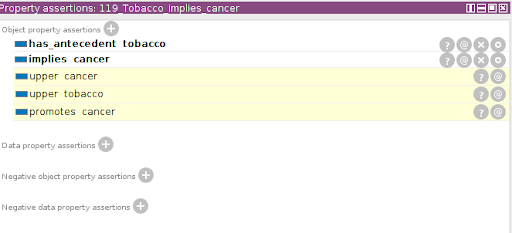
\includegraphics{promotes.png}
	\caption{Example of correct annotation for the \texttt{promotes} relation in Protege}
\label{fig:promotes_example}
\end{figure}

\subsubsection{Suppresses}

Suppresses is the \textbf{opposite} of promotes. Everything valid for promotes
also applies to suppresses, but instead of causes you have
\texttt{does\_not\_cause} and instead of \texttt{implies} you have \texttt{contradicts}.

\paragraph{Declaration}

A declaration is simply a claim stating a domain concept either exists, should
be done or is good/bad. The claim \textit{mafia sells marijuana} is annotated by adding
the \texttt{has\_declaration} with the appropriate domain individual (as seen in figure
\ref{fig:declaration_example}). 

\begin{figure}
	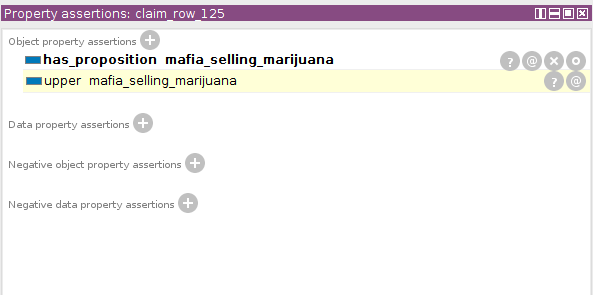
\includegraphics[scale=0.8]{has_declaration.png}
	\caption{Example of correct annotation for the \texttt{has\_declaration} relation in Protege}
\label{fig:declaration_example}
\end{figure}

\subsubsection{Comparison}

Comparisons in debates arise when someone compares two domain individuals,
usually (but not always) by saying one is better according to some feature
(which is a domain individual). The comparison pattern is A is more than B by
C. The domain individual for more is annotated with
\texttt{comparison\_greater}, less is ith \texttt{comparison\_less} and the
optional property of comparison is annotated with
\texttt{comparison\_property}. If there is no property, but an expression like
A is better than B is made, we don’t annotate \texttt{comparison\_property}.
The claim \textit{Alcohol is more influential on the mind than marijuana} is an
example annotated in the figure~\ref{fig:comparison_example}.

\begin{figure}
	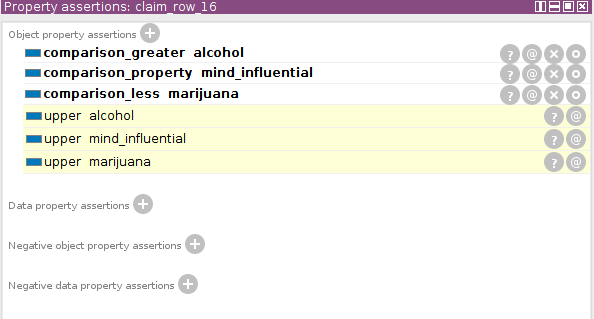
\includegraphics[scale=0.7]{comparison.png}
	\caption{Example of correct annotation for the \texttt{comparison} relation in Protege}
	\label{fig:comparison_example}
\end{figure}

\subsubsection{Step 2.3 Negation}

If you think you need to negate the selected relation, for example in the
sentence: \textit{Marijuana legalization does not promote crime} the author explicitly
states that one domain individual \textbf{does not promote} another. As not promoting \textbf{is
not always} the same as suppresses, we allow you to add negation to any
relation to reflect that. To add negation, simply select ``Negative object
property assertions'' instead of ``Object property assertions'' along with your
relation. Example on the figure \ref{fig:negation_example}. Be \underline{very careful}
when opting for negation, especially with double negation.

\begin{figure}
	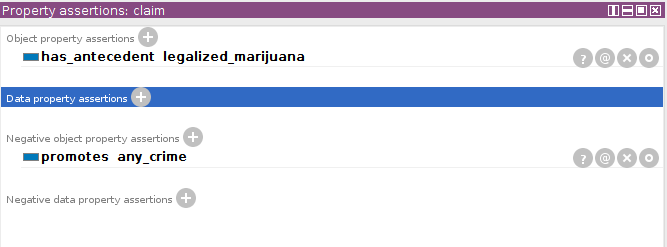
\includegraphics[scale=0.7]{negation.png}
	\caption{Example of correct annotation for negation in Protege}
	\label{fig:negation_example}
\end{figure}

\subsubsection{Step 3 Selecting modality}

We recognize that claims are made in a certain modality (way which they were
expressed with) and discern between:

\begin{itemize}
\item \textbf{Facts}:  believes/argues/thinks that claim C is true (example:
	\textit{Marijuana is legal})
\item \textbf{Policies}: A believes/argues/thinks C should be true in the
	future or should remain true  (example: \textit{Marijuana should be legal}) 
\item \textbf{Value judgement}: A believes/argues/thinks C is morally/ethically
	right or wrong
	\begin{itemize}
	\item Judging of good (example: \textit{Marijuana is great})
	\item Judging of bad (example: \textit{Marijuana sucks})
	\end{itemize}
\end{itemize}
After recognizing the modality, we need to add a property of \texttt{has\_modality} which
can be one of \texttt{fact, policy, good\_value, bad\_value}. 

\subsubsection{Opinion holder}

If the author mentions that his claim is made by someone else, we need to
annotate this information. For example, the following two claims are not made
by the same opinion holder:

\begin{enumerate}
\item Science says marijuana kills people
\item I think marijuana kills people
\end{enumerate}
For the first claim we need to add a property of \texttt{has\_opinion\_holder} to the
claim individual. The opinion holder can be any \textbf{domain individual}. In this
case, the opinion holder is science in claim 1). For claim 2), we don't need to
add a property \texttt{has\_opinion\_holder}, since the default opinion holder is the
author. 

\subsubsection{Step 5 Claim annotation comments}

This is an optional step if you can't annotate the claim for some reason. You
need to annotate the claim individual with a comment if you can't get its
logical form. \textbf{All} claim individuals \textbf{should be annotated with logical form or
commented on}. Adding a comment is done by clicking '+' in the \texttt{Annotations} and
selecting \texttt{rdfs:comment} for a specific claim. If you're missing a domain
individual (see step 1), you can simply write \textit{missing domain individual X},
where X is the domain individual you deem required to get a logical form. 
Figure~\ref{fig:comment_example} shows 
a claim individual, upper pane shows the annotations part where
you can add your comment. 

\begin{figure}
	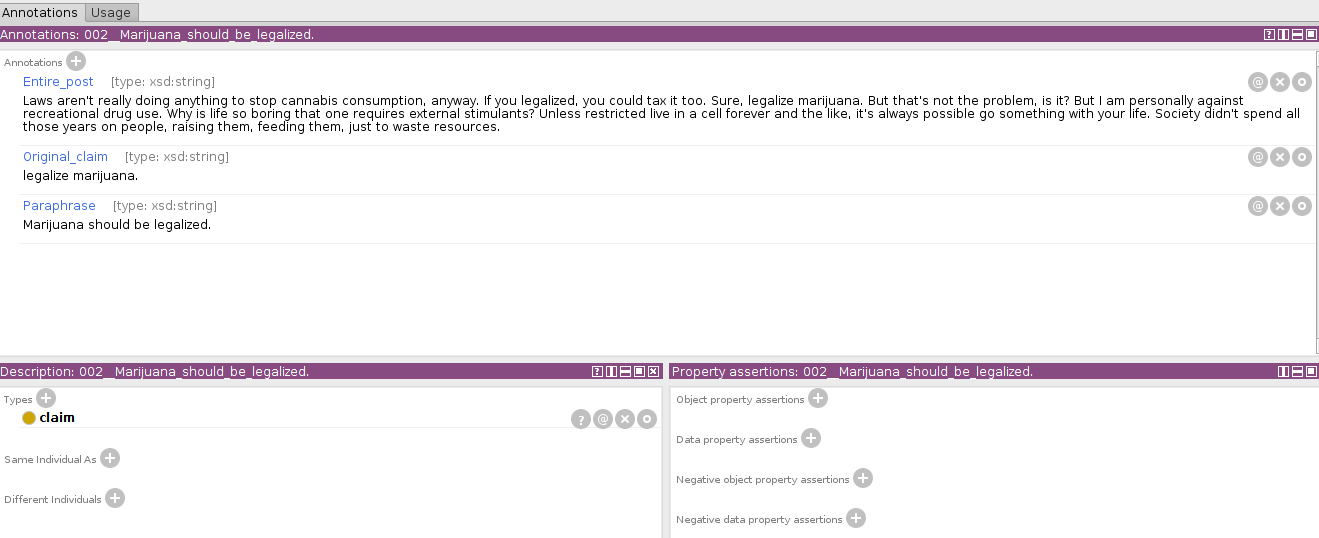
\includegraphics[scale=0.35]{comment.png}
	\caption{Example of correct annotation for adding a comment in Protege}
	\label{fig:comment_example}
\end{figure}

\subsection{Annotation Examples}

\begin{mydef}
 \textit{Marijuana legalization will increase crime rate. }
\end{mydef}

\begin{enumerate}[label=\textbf{Step \arabic*.}, leftmargin=2cm, itemsep=0.5cm]
\item You need to see which domain individuals are mentioned in the claim.
\textit{Marijuana legalization} and \textit{crime rate} are candidate noun phrases which
might be a good place to start. 
\item You see there is a will increase verb and you consult with table in step
2.1. You can narrow down the choice between promotes, implies and
causes as one thing supports another (\textit{marijuana legalization}
and \textit{crime rate}).  
\item To get the modality expressed you can work by elimination. Is there an
estimation if this is good or bad (if so, then value). Is there a
proposal of something that should be done? (if so, policy).
		Otherwise, it’s a factual information. 
\item There seems to be no mention of who is making the claim, so that should
	be the author. 
\end{enumerate}

\noindent Protege steps. 
\begin{enumerate}
\item Select the claim in Protege
\item Enter ``Object property assertions'' depending on the claim pattern identified 
\item Enter: \texttt{has\_antecedent} \texttt{legalized\_marijuana} (Step 1 \& 2)
\item Enter: \texttt{promotes any\_crime} (Step 1 \& 2)
\item Enter: \texttt{has\_modality fact} (Step 3)
\end{enumerate}

\begin{mydef}
Growing marijuana does not make mafia stop selling marijuana.
\end{mydef}

\begin{enumerate}[label=\textbf{Step \arabic*.}, leftmargin=2cm, itemsep=0.5cm]
\item Here we start from domain individuals. Marijuana and mafia related domain
	individuals seem appropriate. Looking into possible options there is a
		domain individual of \texttt{marijuana\_farmer} which seems to be the
		closest to growing marijuana. For mafia, the most similar
		individual seems \texttt{mafia not selling marijuana}
\item  Focusing on the main verb phrase ``does not make'', we can notice the
	pattern A does not cause B, hence we pick \texttt{does\_not\_cause}. We omit the
		rest of the steps as they are similar to example 1. 
\end{enumerate}
Protege steps
\begin{enumerate}
\item Select the claim in Protege
\item Enter “Object property assertions”
\item Enter \texttt{has\_antecedent marijuana\_farmer} (Step 1\&2)
\item Enter \texttt{does\_not\_cause mafia\_not\_selling\_marijuana} (Step 1\&2)
\item Enter \texttt{has\_modality fact} (Step 3)
\end{enumerate}


